\documentclass[../../main.tex]{subfiles}
\graphicspath{{\subfix{../../res/}}}
\begin{document}
The body of literature concerning student dropout is comprehensive, encompassing a range of perspectives from diverse academic disciplines. The issue has been approached through psychological and economic lenses, utilizing both qualitative and quantitative research methods. This section is structured to reflect the various domains and methodologies present in prior studies.

Here is the evolution of the number of publication by year on different publication platform such as Elsevier and Scopus for the terms : \textbf{Predict student success}
\begin{figure}[h!]
    \centering
    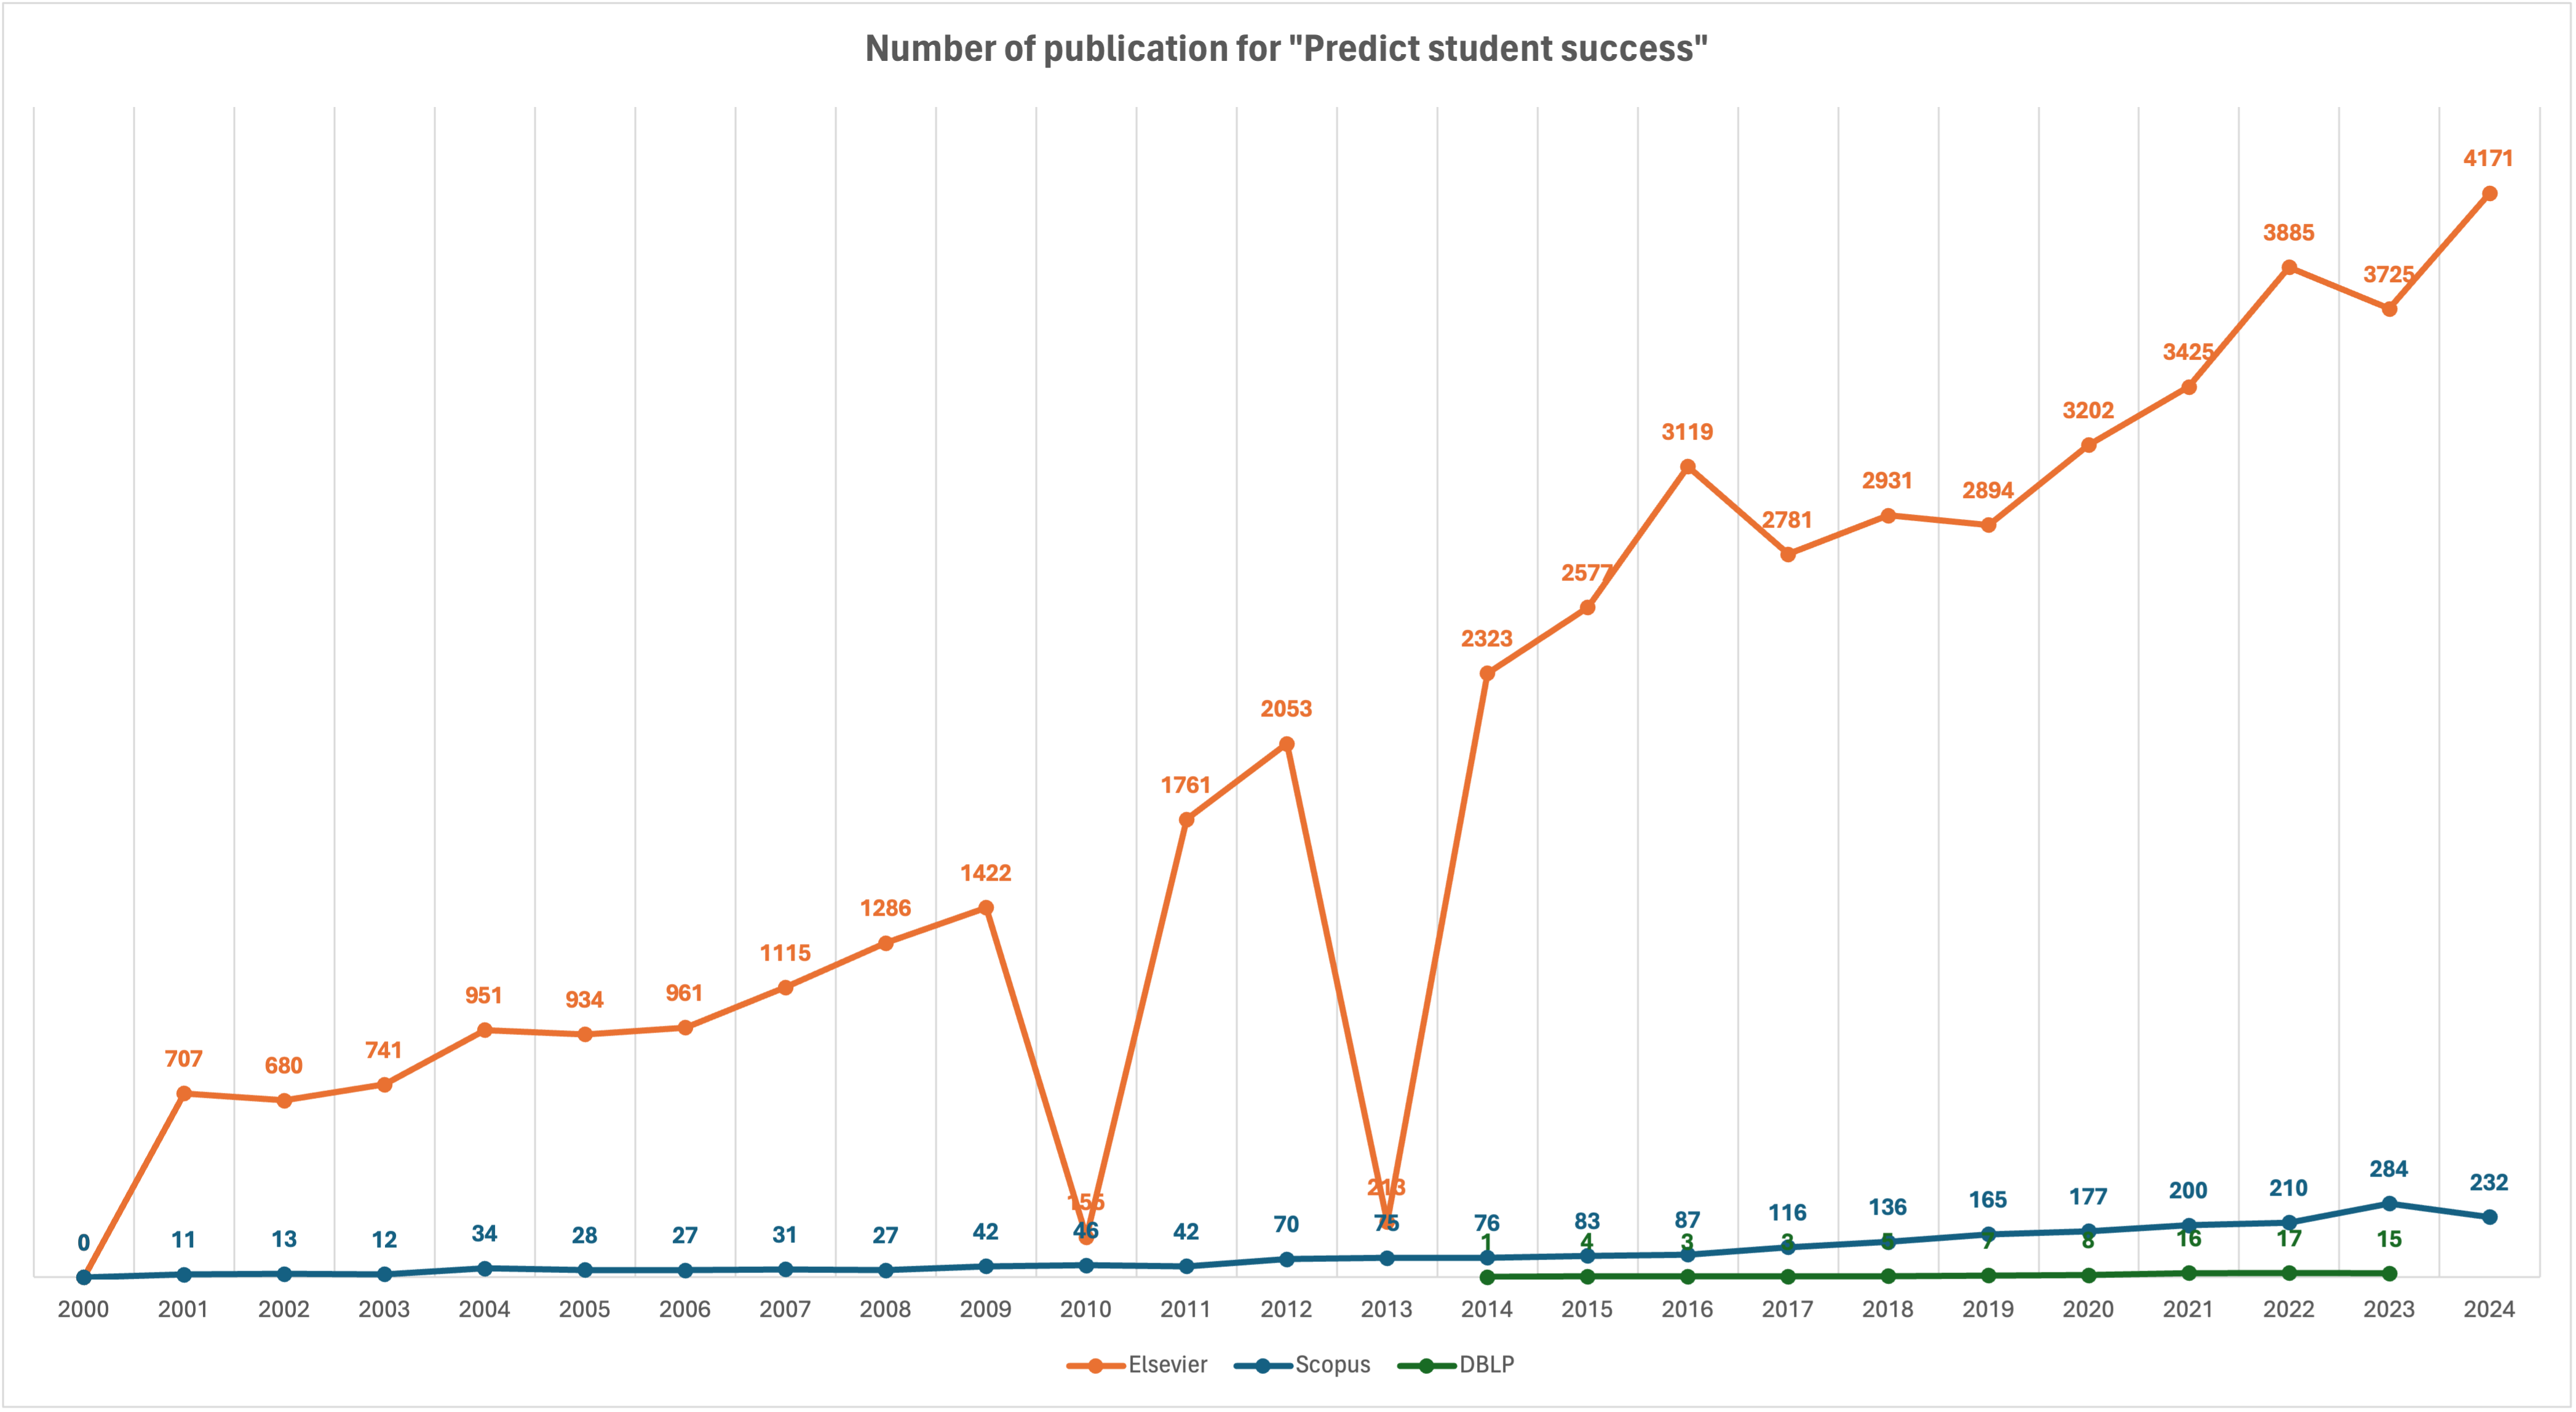
\includegraphics[width=1\linewidth]{res//graph/numberOfPub.png}
    \caption{Number of publication about "Predict student success"}
    \label{fig:nb_pub}
\end{figure}

If we dive deeper into the analytical search on these platform (we are going to concentrate on Scopus for now), using this search term : 
\begin{lstlisting}[breaklines]
TITLE-ABS-KEY ( student  AND dropout )  AND  ( LIMIT-TO ( SUBJAREA ,  "SOCI" )  OR  LIMIT-TO ( SUBJAREA ,  "COMP" )  OR  LIMIT-TO ( SUBJAREA ,  "PSYC" )  OR  LIMIT-TO ( SUBJAREA ,  "ENGI" )  OR  LIMIT-TO ( SUBJAREA ,  "MATH" ) ) 
\end{lstlisting}
We can follow the trend on the number of publication each year about the subject of student dropout prediction and we can also once again notice the longevity of the subject in research, dating all the way back since the 1950's.
Here is the analysis as a graph extracted from Scopus : 
\begin{figure}[H]
    \centering
    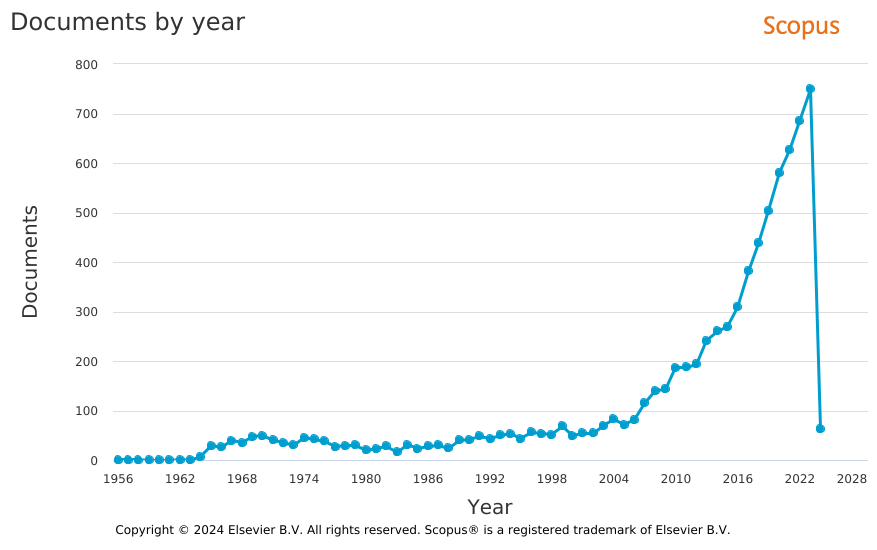
\includegraphics[width=1\linewidth]{res//graph/prediction student/PredictingStudentDropout.png}
    \caption{Evolution of the number of publication per year about \textit{Student dropout prediction}}
    \label{fig:nb_pub_scopus_predictstudent}
\end{figure}

We can also retrieve the number of document \textbf{by country} and \textbf{by subject} :
\begin{figure}[H]
    \centering
    \includegraphics[width=1\linewidth]{res//graph/prediction student/Scopus-Analyze-Country.png}
    \caption{Number of publication by country about \textit{Student dropout prediction}}
    \label{fig:nb_pub_scopus_predictstudent_country}
\end{figure}

\begin{figure}[H]
    \centering
    \includegraphics[width=1\linewidth]{res//graph/prediction student/Scopus-Analyze-Subject.png}
    \caption{Number of publication by subject about \textit{Student dropout prediction}}
    \label{fig:nb_pub_scopus_predictstudent_subject}
\end{figure}

We this understand how universal this problem is from all the different top countries publishing about that subject since the 1950's. At least one country from the five continent have one publication in this subject. Moreover, many fields have looked into the subject, giving us a lot of interesting point of view to analyze from.

Now, if we look for the same subject but adding the \acrshort{ml} or \acrshort{ai} to it :
\begin{lstlisting}[breaklines]
TITLE-ABS-KEY ( student  AND  dropout  AND  ( machine  AND  learning  OR  artificial  AND  intelligence ) )  AND  ( LIMIT-TO ( SUBJAREA ,  "SOCI" )  OR  LIMIT-TO ( SUBJAREA ,  "COMP" )  OR  LIMIT-TO ( SUBJAREA ,  "PSYC" )  OR  LIMIT-TO ( SUBJAREA ,  "ENGI" )  OR  LIMIT-TO ( SUBJAREA ,  "MATH" )  OR  LIMIT-TO ( SUBJAREA ,  "DECI" ) )
\end{lstlisting}

We obtain the following graph :
\begin{figure}[H]
    \centering
    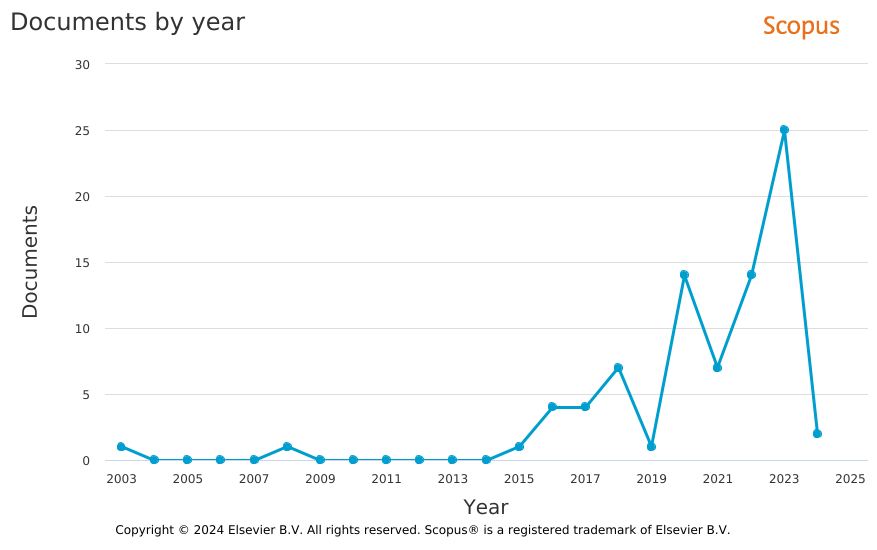
\includegraphics[width=1\linewidth]{res//graph/prediction student with AI/PredictingStudentDropoutW_AI_ML.png}
    \caption{Evolution of the number of publication per year about \textit{Student dropout prediction} including AI or ML}
    \label{fig:nb_pub_scopus_predictstudent_AI}
\end{figure}

Just as before, we have extracted the number of publication by country and by subject :
\begin{figure}[H]
    \centering
    \includegraphics[width=1\linewidth]{res//graph/prediction student with AI/Scopus-Analyze-Country.png}
    \caption{Number of publication by country about \textit{Student dropout prediction \textbf{including AI or ML}}}
    \label{fig:nb_pub_scopus_predictstudent_country_AI}
\end{figure}

\begin{figure}[H]
    \centering
    \includegraphics[width=1\linewidth]{res//graph/prediction student with AI/Scopus-Analyze-Subject.png}
    \caption{Number of publication by subject about \textit{Student dropout prediction \textbf{including AI or ML}}}
    \label{fig:nb_pub_scopus_predictstudent_subject_AI}
\end{figure}


We can see a net evolution of the number of publication over the year. No matter the publication platform, the number of publications on that subject is increasing more or less strongly (mostly dependant on institutions and platform's size and notoriety, which has nothing to do with our research).
This is why studying on the subject is on one hand easy and hard at the same time. Many research have been done, revealing good findings. But the number of difference, from cultural, to temporal to societal is a new challenge to take into account. We will see letter in this study the complexity of creating such a system, not because of technical issue, but human factors.


We've cut this section in two major subsections. The first one, \ref{subsubsec:soa_predictiveapproach}, will review the different ways of analytical analysis on student dropout. These different approaches went from simple adaptation models to economic models and psycho-pedagogic models to predict and describe student dropout. Then, in \ref{subsubsec:soa_predictiveapproach} we are going to study different mathematical algorithms and models and use ML models to predict student dropout.

It is interesting to look at the opposite side of the "problem" to gather which information have been used to predict student dropout. We could then hypothesise and extrapolate about if for one student it could predict its failure and for another its success.
However, some factors cited are sensibly comprehensible about one's failure (for example, it is logical that a student with health and family problem will have a greater probability of failure.) However, even with a good situation, one can be uninterested in its formation of choice and then dropout. 
What we want to filter and understand from the literature is factors that could lead us to the potential intellect of student such as their hobbies, past experience in the domain, motivation.

But first, let's define success and what is a student choice. 

\end{document}